% The beamer document type for presentations
\documentclass[inputenc]{beamer}

% Import the packages
\usepackage{graphicx}
\usepackage{tikz}
\usepackage{url}
%\usepackage{hyperref}

% Set the colors of the URL links
\hypersetup{
    colorlinks=true,
    linkcolor=blue,
    urlcolor=purple,
}

% This adds the table of contents before each section
\AtBeginSection[]
{
  \begin{frame}<beamer>
  \frametitle{Outline}
  \tableofcontents[currentsection]
  \end{frame}
}
  
\title[Introduction to LaTeX]{\huge Introduction to \LaTeX{}}
\author{Aleix Lafita}
\institute{Bateman group (EMBL-EBI)}
\date{16th October 2018}

\begin{document}

\begin{frame}
  \titlepage
  \centering
  
\includegraphics[width=0.4\textwidth]{embl_logo}
\end{frame}

\begin{frame}{Outline}
    \tableofcontents
\end{frame}

%%%%%%%%%%%%%%%%%%%%%%%%%%%%%%%%%%%%%%%%%%%%%%%%%%%%%%%%%%
\section{Introduction}

\subsection{Pros and Cons}

\begin{frame}{Pros and Cons}
    PROS
    \begin{itemize}
        \item Structured documents with consistent formatting
        \item Version control (e.g. \texttt{Git} integration)
        \item High quality graphics
        \item Mathematical equations and formulas
        \item Table of contents, footnotes, references and bibliography
        \item Portable to any platform and collaborative
        \item Free and open source
    \end{itemize}
    \vspace{0.5cm}
    CONS
    \begin{itemize}
        \item Steep learning curve, not intuitive
        \item Customization can be difficult
        \item Danger to overcomplicate things
    \end{itemize}
\end{frame}

\begin{frame}{History of \LaTeX{}}
    
    \textbf{When?} \TeX{} was released in 1977, before Microsoft Word (1983).
    
    \vspace{0.5cm}
    \textbf{Why?} Control the arrangement of text and graphics in documents. 
    
    \begin{figure}
        \centering
        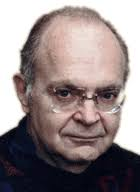
\includegraphics[width=0.25\textwidth]{knuth}
        \caption{Donald Knuth, the creator of \TeX{}. \footnote{Source: \href{https://www-cs-faculty.stanford.edu/~knuth}{Stanford University}}}
    \end{figure}
    
\end{frame}

\subsection{The \LaTeX{} system}

\begin{frame}{The \LaTeX{} system}

\LaTeX{} (pronounced "lay-tech" or "lah-tech") is a document preparation system. 

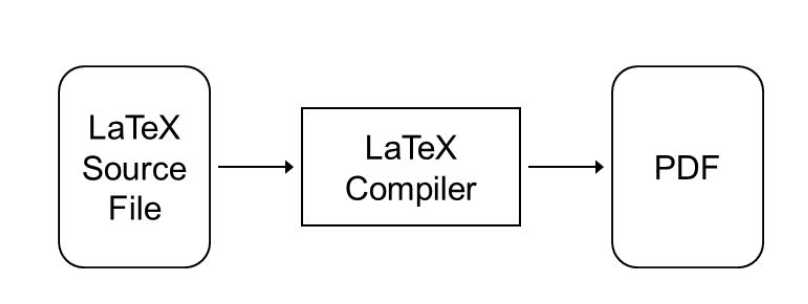
\includegraphics[width=\textwidth]{latex_system.png}

%Instead of visually formatting your text, you enter your manuscript text intertwined with \Tex{} commands in a plain text file. You then run \Tex{} to produce formatted output, such as a PDF file. Thus, in contrast to standard word processors, your document is a separate file that does not pretend to be a representation of the final typeset output, and so can be easily edited and manipulated.

\end{frame}

\subsection{Terminology}

\begin{frame}{Terminology}
    
    \begin{itemize}
        \item \textbf{Format:} the syntax you type in your source file (\TeX{}, \LaTeX{})
        \item \textbf{Engines/Compilers:} what creates the PDF from your text file (pdf\LaTeX{}, Xe\LaTeX{}, Lua\TeX{})
        \item \textbf{Distributions:} software that bundles everything for download (\TeX{} Live, MiK\TeX{})
        \item \textbf{Online editors:} websites that allow you to edit and compile \LaTeX{} (ShareLaTeX, Overleaf)
    \end{itemize}
    
    \vspace{1cm}
    
    \centering
    \url{https://www.tug.org/levels.html}
    
\end{frame}

\begin{frame}{Obtain this presentation!}

    \centering
    
\includegraphics[width=0.5\textwidth]{overleaf_QR}
    
    \url{https://goo.gl/ECAVZb}
    
\end{frame}

%%%%%%%%%%%%%%%%%%%%%%%%%%%%%%%%%%%%%%%%%%%%%%%%%%%%%%%%%%
\section{Hands on}

\subsection{Your first \LaTeX{} document}

\begin{frame}{Your first \LaTeX{} document}
    
    
\includegraphics[width=\textwidth]{overleaf_website.png}
    
    \centering
    \url{https://www.overleaf.com}
    
\end{frame}

\begin{frame}{Your first \LaTeX{} document}
    
    Create a document and add the following:
    \begin{enumerate}
        \item Add metadata: title, auhtor, date \url{https://www.overleaf.com/learn/latex/Creating\_a\_document\_in\_LaTeX}
        \item Emphasize text \url{https://www.overleaf.com/learn/latex/Bold,\_italics\_and\_underlining}
        \item Insert a figure \url{https://www.overleaf.com/learn/latex/Inserting\_Images}
        \item Add references \url{https://www.overleaf.com/learn/latex/Bibliography\_management\_with\_natbib}
    \end{enumerate}
    
    \vspace{0.5cm}
    Solution: \url{https://www.overleaf.com/read/ybnfpbdzfjvm}
    
\end{frame}

\subsection{Your thesis in \LaTeX{}}

\begin{frame}{Your thesis in \LaTeX{}}
    
    Time to have some FUN! Be creative...
    
    \vspace{1cm}
    Thesis template:
    \url{https://www.overleaf.com/1449587773cvpcrtntgjwr}
    
    \vspace{1cm}
    If in trouble, consult the \texttt{Thesis in} \LaTeX{} tutorial: 
    \url{https://www.overleaf.com/learn/latex/How_to_Write\_a\_Thesis\_in\_LaTeX\_(Part\_1):\_Basic\_Structure}
    
\end{frame}

%%%%%%%%%%%%%%%%%%%%%%%%%%%%%%%%%%%%%%%%%%%%%%%%%%%%%%%%%%
\section{Bright future}

\subsection{Recommendations}

\begin{frame}{Recommendations}

    \begin{itemize}
        \item Start small!
        \item Stay simple - do I really need that?
        \item Don't lose your faith in Donald Knuth
        \item Do not try to understand everything when using templates
        \item The internet is wise and has the answers you desire
    \end{itemize}
    
\end{frame}

\subsection{Additional materials}

\begin{frame}{Additional materials}

\begin{itemize}
    \item Most of the introduction is based on \texttt{The Not So Short Introduction to} \LaTeX{}, which covers other advanced topics:
    
    {\small\url{http://tug.ctan.org/info/lshort/english/lshort.pdf}}
    \item \texttt{Thesis writting in} \LaTeX{} created by predocs at the EBI: \url{https://github.com/EBI-predocs/latex-thesis}
    
    \item \TeX{}\texttt{ Live}: download \LaTeX{} command line to your computer \url{https://www.tug.org/texlive}
    
    \item \TeX{}\texttt{works}: Desktop editor and working environment \url{http://www.tug.org/texworks}
    
\end{itemize}

\end{frame}

\end{document}
